\section{Tabs}

\begin{figure}[H]
\centering
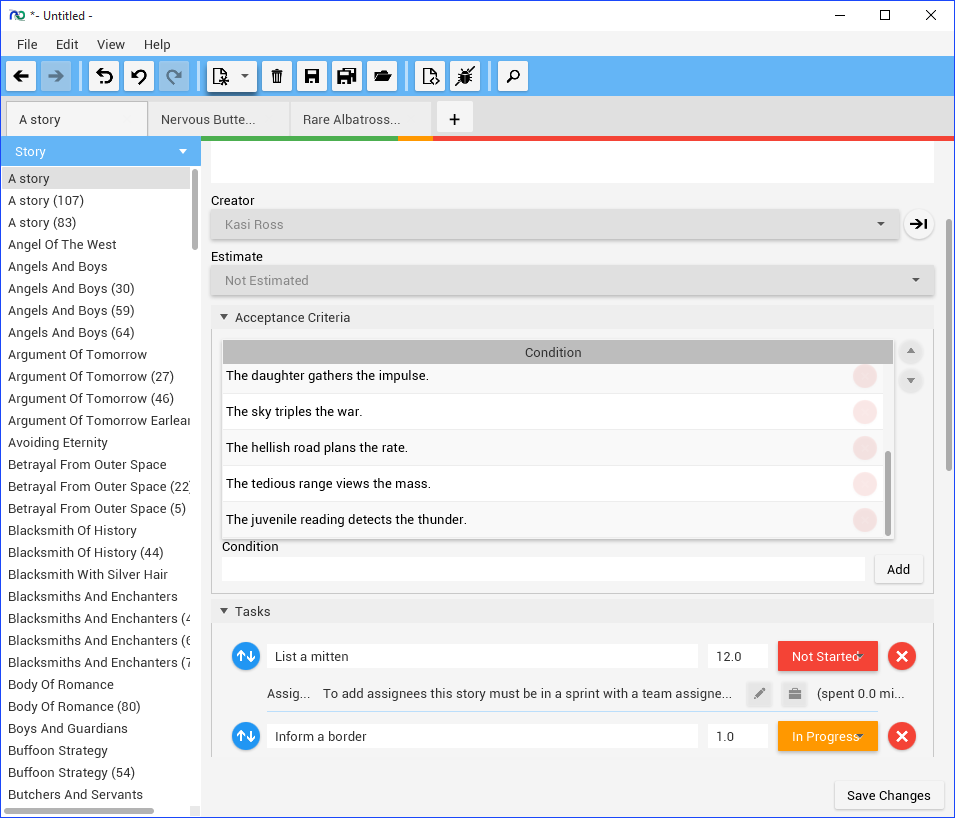
\includegraphics[width=\textwidth]{images/screenshots/tabs1.png}
\caption{Tabs}
\label{fig:revert}
\end{figure}

To make your life easier, murcs provides tab management functionality. To open something in a new tab, CTRL + Click on the it. You can open new tabs with the "+" button or by pressing CTRL + T. Close tabs with the close button or by pressing CTRL + W


You can rearrange tabs by clicking on the tab header and dragging the tab around. If you drop the tab on the tab header the tabs will be reordered.

\begin{figure}[H]
\centering
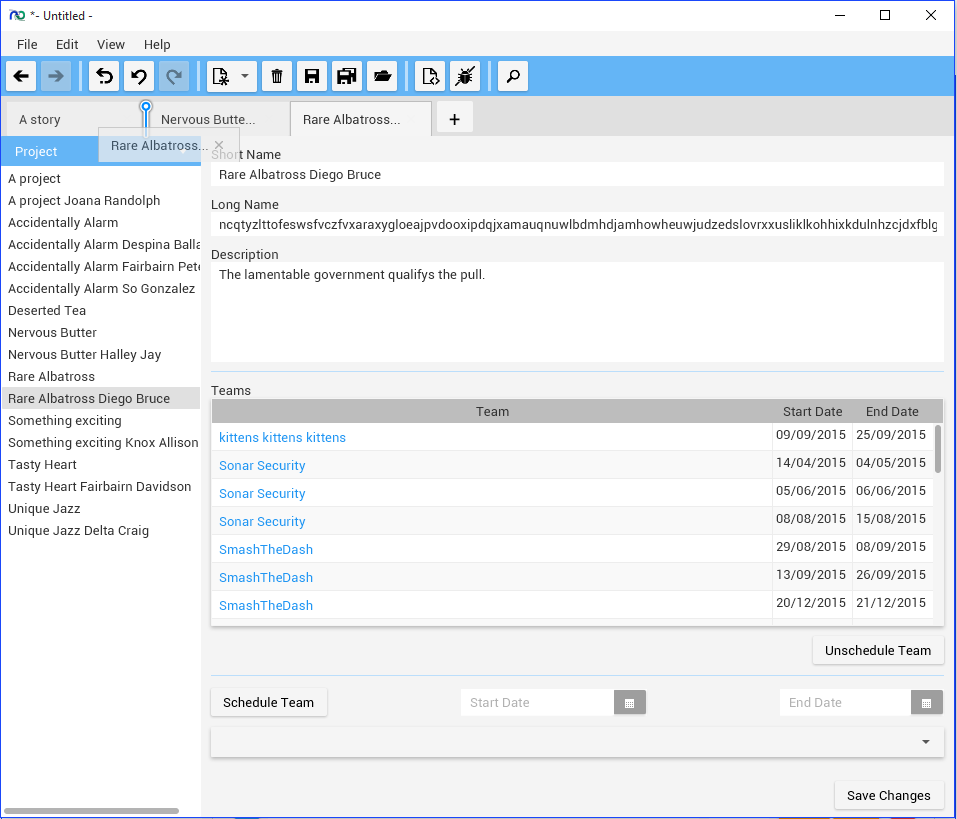
\includegraphics[width=\textwidth]{images/screenshots/tabs2.png}
\caption{Reordering Tabs}
\label{fig:revert}
\end{figure}

If you drop the tab somewhere else, a new window will be opened with the tab in it. You can also move tabs between windows.

\begin{figure}[H]
\centering
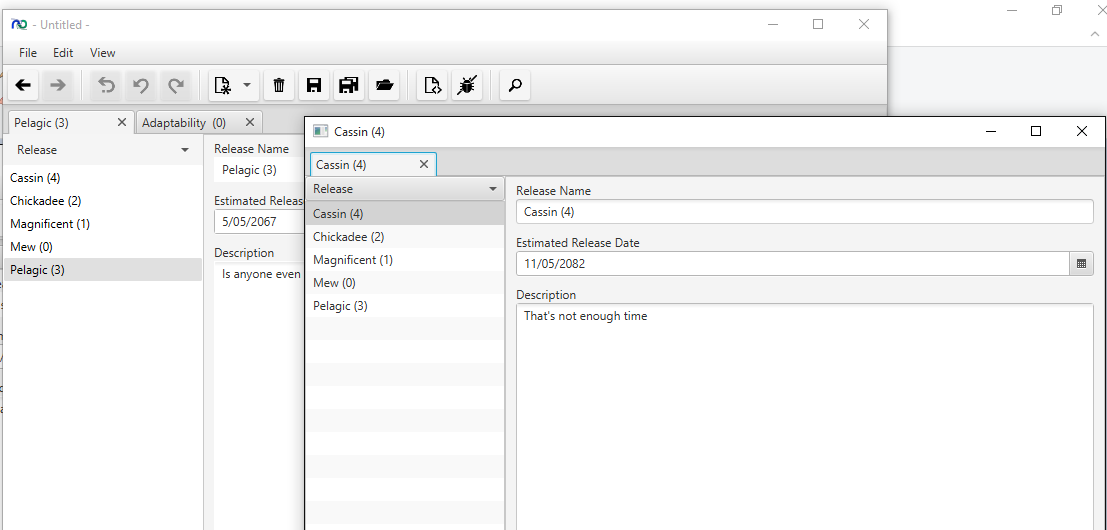
\includegraphics[width=\textwidth]{images/screenshots/tabs3.png}
\caption{Opening a new window}
\label{fig:revert}
\end{figure}

You can't close all the windows in the main view. If you do, a new tab will be automatically opened.